\chapter{Background}
\label{ch:Background}

In this chapter, I present the concepts relevant to the subject of the thesis. First, I introduce the topic of MT and the type of architecture I focus on later in the work. Next, I outline the problem of ambiguity and bias in MT models.

% WSD (if I end up using it)
% QE (if I end up using it)

%%%%%%%%%%%%%%%%%%%%%%%%%%%%%%%%%%%%%%%%%%%%%%%%%%%%%%%%%%%%%%%%%%%%%%%%%%%%%%%%%%%%%%%%%%%%
\section{Neural Machine Translation}
\label{sec:Background:NMT}

Machine Translation (MT) is the process of using computer technology to translate text from one natural language to another. This can be achieved using different paradigms. There are three main types of machine translation systems: Rule-based Machine Translation (RBMT), Statistical Machine Translation (SMT) and Neural Machine Translation (NMT). 

Conventional RBMT systems use pre-defined rules based on syntax, morphology and semantics, created by professional linguists. Since language is dynamic and evolves over time, these rules need frequent adaptation, which is costly. However, the key weakness of rule-based translation systems is that they require extensive lexicons and a large set of rules \parencite{SMT_book}. 

SMT systems, on the other hand, use a data-driven approach that utilizes statistical models derived from the analysis of bilingual and monolingual corpora. The quality of SMT output depends heavily on the size and quality of the corpora used to train the models. SMT’s general weakness is that it can only translate a phrase if it exists in the training dataset \parencite{SMT_book}.

Neural Machine Translation (NMT) is a subfield of SMT, which uses an artificial neural network to learn a statistical model for machine translation. Unlike traditional SMT systems, which require a pipeline of specialized components such as language model and translation model, NMT trains its statistical model end-to-end, mapping directly from an input source language to an output target language. NMT can recognize patterns in the training data to determine a context-based interpretation that can predict the likelihood of a sequence of words. Unlike SMT, NMT models are able to learn from each translation task and improve upon each subsequent translation. NMT models are more memory-efficient and also have a higher accuracy than SMT models, which makes them the appropriate choice for creating high-quality MT systems \parencite{NMT_book}.

% TODO: How in deep should I explain the Transformer and NMT?

%%%%%%%%%%%%%%%%%%%%%%%%%%%%%%%%%%%%%%%%%%%%%%%%%
\subsection{Sequence-to-Sequence Modeling}
\label{sec:Background:Seq2Seq}
The task of NMT is typically solved using Sequence-to-Sequence (Seq2Seq) modeling \parencite{seq2seq}. A Seq2Seq model has two parts: an encoder and a decoder. Both work separately and come together to form a large neural network model. This architecture has the ability to handle input and output sequences of variable length. A simplification of the architecture of NMT models can be seen in Fig. \ref{fig:seq2seq}. Firstly, each word in the input sentence is fed separately into the encoder to encode the source sentence into an internal fixed-length representation called the context vector. This context vector contains the meaning of the sentence. Secondly, the decoder decodes the fixed-length context vector and then predicts the output sequence.

\begin{figure}
  \centering
  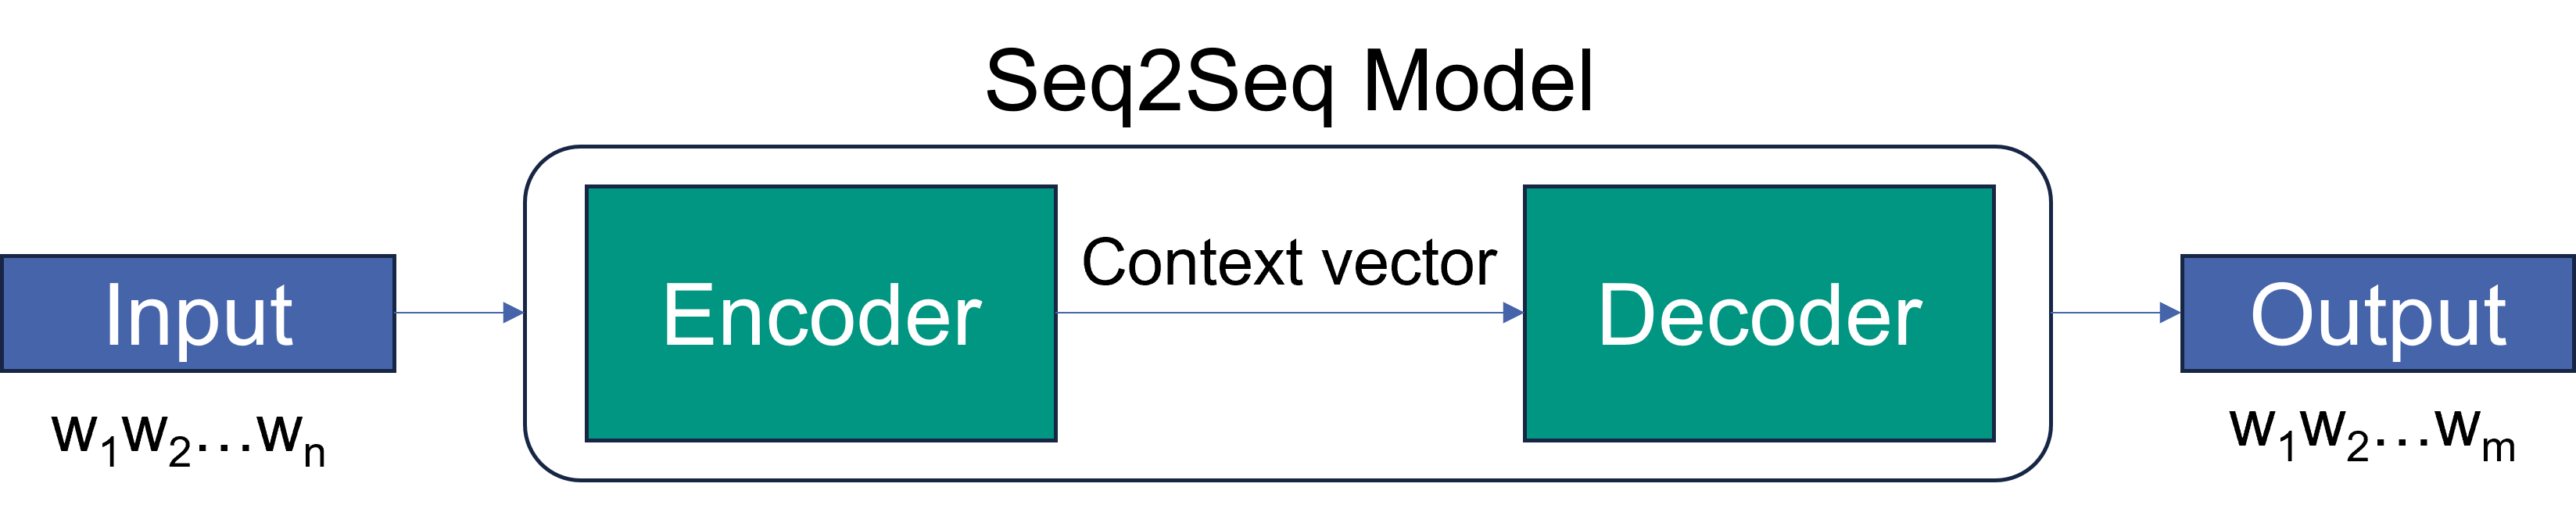
\includegraphics[scale=0.57]{figures/seq2seq.png}
  \caption{Sequence-to-Sequence Modeling}
  \label{fig:seq2seq}
\end{figure}

The original architecture consists of a pair of Recurrent Neural Networks (RNNs) in the roles of encoder and decoder. RNNs process the input sequence token by token, which prohibits parallelization and makes the training and inference slow, especially when processing longer sequences. Also, they suffer from vanishing or exploding gradients, which is inconvenient for effective training. One solution for these problems served Long Short-Term Memory (LSTM) networks, a type of RNN that has additional memory gates to regulate the flow of information through the network better \parencite{lstm}. Despite this, using a fixed-length context vector still incurs a bottleneck in the model. To alleviate this problem, the use of attention-based architectures for neural machine translation was explored \parencite{attention}. 

The attention mechanism allows the decoder to look at the source tokens that are relevant while generating the next token. Despite all these efforts, using RNN-based encoder and decoder still forces the network to handle input sequentially, which makes it difficult to handle long-range dependencies within the input and output sequences from memory. Hence, \cite{transformer} proposed the Transformer architecture, which replaces RNNs with self-attention layers in the Encoder-Decoder network. Since in this work I make use of models based on the Transformer, next I will introduce its basic principle and components.

%%%%%%%%%%%%%%%%%%%%%%%%%%%%%%%%%%%%%%%%%%%%%%%%%
\subsection{Transformer Architecture}
\label{sec:Background:Transformer}
A Transformer is a Seq2Seq model, introduced by \citet{transformer}. An important feature of the Transformer architecture is its attention mechanism. The attention module looks at an input sequence and decides at each step which other parts of the sequence are important, differentially weighting the significance of each part of the input data. Like RNNs, Transformers are designed to handle sequential input data, such as natural language. However, unlike RNNs, Transformers can process the whole input sequence in parallel. The attention mechanism provides context for any position in the input sequence. This feature allows for more parallelization than RNNs and therefore reduces training times significantly \parencite{transformer}.

% Transformer Components
The Transformer architecture as presented in the original paper by \citet{transformer} is depicted in Fig. \ref{fig:transformer}.
The input embedding layer converts the high-dimensional input sequence into a low-dimensional sequence of vectors to capture the meaning and context.
The positional encoding preserves the sequential order of words in the input sentence and can be thought of as the distance of one word to another word in a sequence. This relative position of the words in the sequence is needed since the words are passed in parallel, as opposed to RNNs, which process them in order.
Self-attention is the weighted sum of all other words in the input sequence for each word using similarity (dot product) and SoftMax to focus on the most relevant parts of the input for each element. The multi-head attention repeats self-attention multiple times based on how many encoder/decoder layers there are.

There are multiple encoder and decoder layers. 
Each encoder has one multi-head self-attention, which encodes the weight of the input words to each other. 
Each decoder has one masked multi-head self-attention and one multi-head attention. The masked multi-head self-attention ensures that only words coming before a word are compared to that word, which means it only attends to preceding words in the input sequence during the decoding process. Applying a mask forces the model to ignore future words and focus only on the preceding words during the attention computation. % The mask specifically sets the attention weights to a very large negative value for the positions that correspond to future words, effectively making those weights close to zero after applying the softmax function. 
The multi-head cross-attention module in the decoder compares output tokens to input tokens.
Both the encoder and the decoder have one feed-forward layer, as well as adding and normalizing of residuals at each stage after the attention layers.

The output from the decoder is a vector of length of the input tokens. This output is fed into a fully connected (linear) layer to map it to a set of output prediction and then converted into probability over possible words like multi-class classification using a SoftMax layer.


The Transformer revolutionized NMT by replacing recurrence with attention, which allowed for simultaneous computations and more effective handling of long-range dependencies. This makes them efficient on hardware like GPUs and TPUs and pushes them to be the rational choice for architecture in the realm of MT.

\begin{figure}
  \centering
  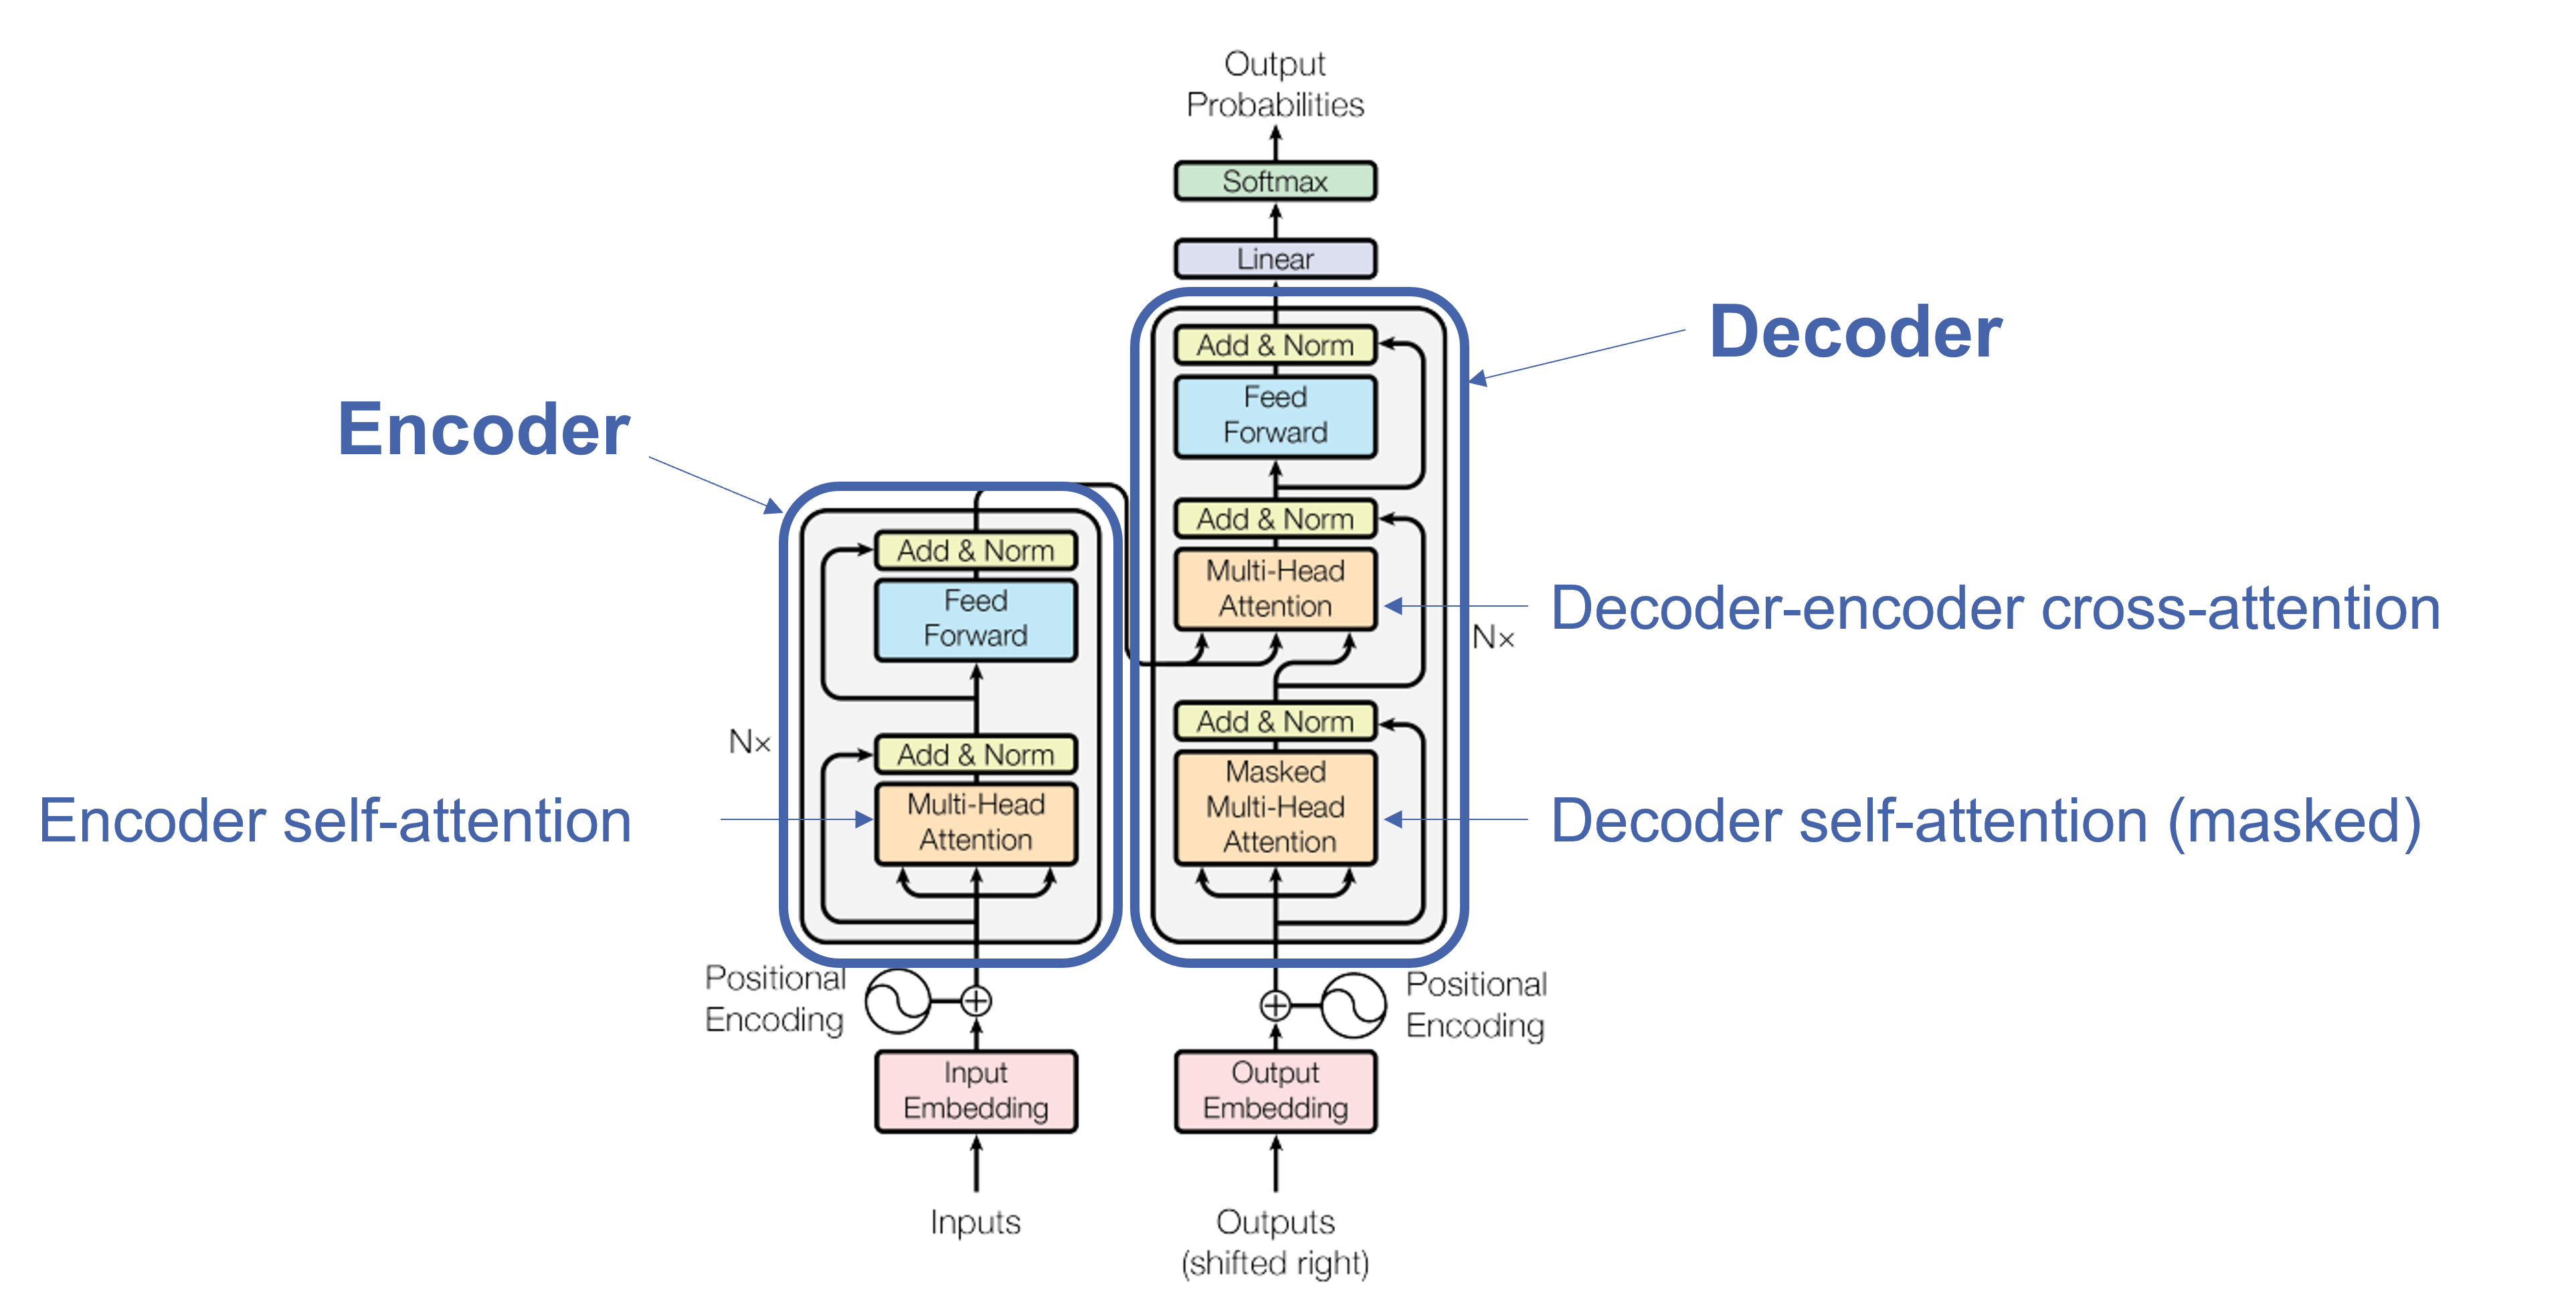
\includegraphics[scale=0.5]{figures/transformer.png}
  \caption{The Transformer Architecture}
  \label{fig:transformer}
\end{figure}

% Explain autoregressive sampling?

%%%%%%%%%%%%%%%%%%%%%%%%%%%%%%%%%%%%%%%%%%%%%%%%%%%%%%%%%%%%%%%%%%%%%%%%%%%%%%%%%%%%%%%%%%%%
\section{Ambiguity and Bias in Machine Translation}
\label{sec:Background:Ambiguity_Bias}
Biases present in AI systems are an important problem stemming from cultural and historical issues present in the data from which models are learning. The developed systems in turn reinforce the present societal prejudices and old social norms, instead of mitigating them. 
It is important to understand how these biases occur in translation and to differentiate the different types of bias one may face.

Next, I will define the concepts of ambiguity and bias.

%%%%%%%%%%%%%%%%%%%%%%%%%%%%%%%%%%%%%%%%%%%%%%%%%
\subsection{Ambiguity}
\label{sec:Background:Ambiguity}
Ambiguity refers to the quality of being open to more than one interpretation, as in not having one obvious meaning. It is the type of meaning in which a phrase, statement, or resolution is not explicitly defined, making several interpretations plausible. A common aspect of ambiguity is uncertainty. In MT, ambiguity occurs when the source text leaves some essential properties unspecified, but the target language requires the property to be specified for correct translation. 

The ambiguity can be \textbf{resolvable} or \textbf{unresolvable}. It is resolvable when some semantic property required for the subject to be disambiguated can be found in the context, which defines the rest of the text available to the translation system. On the other hand, it is unresolvable, when no property necessary for disambiguation can be inferred from the context. To illustrate these two cases, we will look at two examples. When translating the sentence "She is a doctor." from English to German, which has no gender-neutral word for "doctor", the translation system has to choose the male ("Arzt") or female ("Ärztin") gender word for "doctor". In this case, the word "doctor" is ambiguous. However, the gender is resolvable from context due to the presence of the female pronoun "she". In contrast, the example sentence "I am a doctor." also contains the ambiguous word "doctor", but it is not indicated in the rest of the text whether the intended referent of "I" and "doctor" is a man or a woman. This makes the ambiguity in this case unresolvable \parencite{bias_taxonomy}.

When the ambiguity is unresolvable, the translation system cannot make an informed decision and instead applies randomness or previously acquired knowledge in choosing the translation, making an \textbf{unjustified assumption}. The assumption is unjustified because nothing actually present in the source text justifies it. In the example of "I am a doctor." the translator typically decides for the male translation of the word "doctor", because this case appears most often in similar contexts in its training data. Although, context allows for two possible translations in German for the ambiguous word "doctor", the system will consistently prefer the male translation, which leads to a \textbf{bias}. 

%%%%%%%%%%%%%%%%%%%%%%%%%%%%%%%%%%%%%%%%%%%%%%%%%
\subsection{Bias}
\label{sec:Background:Bias}
Bias refers to a disproportionate weight in favor of or against an idea or thing, usually in a way that is closed-minded, prejudicial, or unfair. In machine translation, it is the tendency to discriminate against certain individuals or groups in favor of others. Biases typically stem from unresolved ambiguities leading to unjustified assumptions, and can be classified as follows \parencite{bias_taxonomy}:
\begin{itemize}
    \item \textbf{Gender bias}: This type of bias occurs when there is an unresolvable ambiguity relating to the gender of people. Some commonly gender ambiguous words are professions such as doctor, teacher, cleaner. 
    \item \textbf{Number bias}: This bias presents itself when the English pronoun "you" has an unresolvable ambiguity concerning whether it refers to a single person ("du" in German) or multiple people ("ihr" in German). 
    \item \textbf{Formality bias}: This bias occurs when the English pronoun "you" has an unresolvable ambiguity concerning whether the subject is addressed formally ("Sie" in German) or informally ("du" in German). 
\end{itemize}

A MT system is biased if, while dealing with unresolvable ambiguities and deciding which unjustified assumptions to make, its decisions are not random. This means that the system makes certain unjustified assumptions more often than others. For example, if it consistently translates the occupation "doctor" as male, then the translator is biased \parencite{bias_taxonomy}.

Furthermore, biases can lead to harmful results. These can be categorized into representational and allocational harms \parencite{Savoldi_2021}. \textbf{Representational harms} detract from the representation of social groups and their identity and can be further distinguished into \textit{under-representation} and \textit{stereotyping}. Under-representation refers to the reduction of the visibility of certain social groups through language, such as producing a disproportionately low representation of women (e.g., most feminine entities in a text are misrepresented as male in translation) and not recognizing the existence of non-binary individuals (e.g., when a system does not account for gender-neutral forms). Stereotyping regards the propagation of negative generalizations of a social group, for example, belittling feminine representation to less prestigious occupations (e.g. teacher (feminine) vs. lecturer (masculine)). \textbf{Allocational harms} occur when a system allocates or withholds opportunities or resources to certain groups, for example, when a woman attempting to translate her biography by relying on an MT system requires additional energy and time to revise incorrect masculine references \parencite{Savoldi_2021}. In the long run, stereotypical assumptions and prejudices are reinforces and affect the self-esteem and behavior of members of the target group, and may also influence indirect stakeholders. 

%%%%%%%%%%%%%%%%%%%%%%%%%%%%%%%%%%%%%%%%%%%%%%%%%
\subsection{Language Types Based on Gender}
\label{sec:Background:Language}
Currently, most of the scientific literature around biases in MT focuses on gender bias \parencite{Savoldi_2021}. In order to understand gender bias better, we need to know how it is encoded linguistically (lexical, pronominal, grammatical). There are three main groups relating to the linguistic form of gender \parencite{Savoldi_2021}:
\begin{itemize}
    \item \textbf{Genderless languages} (e.g., Finnish, Turkish): have minimal expression of gender, relating only to lexical gender (e.g., in Finnish "sisko" (sister) and "veli" (brother)).
    \item \textbf{Notional gender languages} (e.g., English, Danish): in addition to lexical gender (mom/dad) have also pronominal gender expression (she/he, her/him).
    \item \textbf{Grammatical gender languages} (e.g., Spanish, Arabic): each noun is assigned to a class such as masculine, feminine or neutral. Grammatical gender is expressed morphosyntactically, such that several parts of speech beside the noun (e.g., verbs, determiners, adjectives) carry gender inflections.
\end{itemize}

To illustrate the difference between the different groups with an example, we look at the English sentence "He/She is a good friend.". This sentence has no expression of gender in a genderless language like Finnish ("Hän on hyvä ystävä."), whereas in Spanish several masculine or feminine forms are needed to express the gender ("El/Ela es un/una buen/buena amigo/amiga."). 

Previous scientific work around bias has focused on detection and mitigation of bias in NMT models using various techniques, which I will present in the following two subsections.  % For more information, \citet{Savoldi_2021} provide a more extensive literature review on the topic of gender bias in MT, critically reviewing current conceptualizations of bias in light of theoretical insights from related disciplines. 

%%%%%%%%%%%%%%%%%%%%%%%%%%%%%%%%%%%%%%%%%%%%%%%%%
\subsection{Bias Detection}
\label{sec:Background:Bias_Detection}

Dedicated benchmarks, evaluations, and experiments have been designed in order to assess the existence and scale of gender bias across several languages. In MT, several studies concerned themselves with pronoun translation and coreference resolution across typologically different languages. 

For example, \citet{Prates_2019} investigate pronoun translation from 12 genderless languages into English. They retrieve around 1,000 job positions from the U.S. Bureau of Labor Statistics and build synthetic examples like the Hungarian "Ö egy mernök." ("He/She is an engineer."). Then they use the Google Translate API to generate translations and gather statistics about the frequency of female, male and gender-neutral pronouns in the translated output. By comparing the proportion of pronoun predictions against the real-world proportion of men and women employed in 22 sectors, they find that the MT system not only exhibits a strong tendency toward male defaults, but it also underestimates feminine frequency at a greater rate than occupation data alone suggest, failing to reproduce a real-world distribution of female workers.

Similarly, \citet{Cho_2019} extend the analysis to Korean-English including both occupations and sentiment words such as "kind". Since the samples are ambiguous by design, the predictions of he/she pronouns are expected to be random, but masculine pronouns seem to appear more often. \citet{Cho_2019} also make light of the fact that a higher frequency of feminine pronoun translations does not necessarily reflect a bias reduction. In some cases, it may be an indication for stereotyping, such as associating nurse more often with feminine. Therefore, while frequency count may be suitable for testing under-representational harms, it may ignore stereotyping.

Expanding beyond synthetic examples and sentiment word phrases, \citet{Gonen_2020} develop a novel technique to mine examples from real-world data to explore gender issues. They inspect the translation of natural yet ambiguous English sentences into four grammatical gender languages (Russian, German, Spanish and French) from three language families (Slavic, Germanic and Romance). Their analysis of the ratio and type of generated masculine/feminine job titles consistently exhibits social asymmetries, such as translating "lecturer" as masculine and "teacher" as feminine.

Furthermore, \citet{Stanovsky_2019} present the first challenge set and evaluation protocol for the analysis of gender bias in MT. Challenge sets are artificially created, usually small datasets that represent some gender-related issue, such as assigning the right pronoun to a specific role. Their purpose is to isolate the impact of gender from other factors that may affect the performance of the NMT system. Also, automatic evaluation methods for bias are needed, because the BLEU score, normally used for assessing the quality of translations, cannot judge on the occurrence of bias. 

For building the challenge set called WinoMT, \citet{Stanovsky_2019} used data introduced by two recent coreference gender-bias studies: Winogender \parencite{Rudinger_2018_coreference} and WinoBias \parencite{Zhao_2018_coreference}. They are composed of English sentences which cast participants into non-stereotypical gender roles (e.g., “The doctor asked the nurse to help \textit{her} in the operation.”). WinoMT is equally balanced between male and female genders, as well as between stereotypical and non-stereotypical gender-role assignments (e.g., a female doctor versus a female nurse). 
For assessing gender bias in translating the challenge set, \citet{Stanovsky_2019} devise an automatic gender bias evaluation method for eight target languages with grammatical gender, based on morphological analysis (e.g., the use of female inflection for the word “doctor”). They use the developed method to evaluate four popular industrial MT systems and two recent state-of-the-art academic MT models, measuring gender accuracy, difference in performance between male and female, difference in performance between stereotypical and non-stereotypical gender role assignments. An important discovery the authors made was that MT systems are faulty to the point of actually ignoring explicit feminine gender information in source English sentences. For example, MT systems produce a wrong masculine translation of the job title "baker", although it is referred to by the pronoun "she".

\citet{Hovy_2020} speculate that the existence of age and gender stylistic bias may be due to under-exposure of MT models to the writings of women and younger people. They test this assumption by automatically translating a corpus of online reviews with available metadata about users. Then, they compare this demographic information with the prediction of age and gender classifiers run on the MT output. The results prove that different commercial MT models systematically make authors appear older and male.

\citet{MuST-SHE} develop the MuST-SHE corpus, a natural benchmark for three language pairs (English-French/Italian/Spanish). Unlike challenge sets, natural corpora quantify whether MT yields reduced feminine representation in real-world scenarios and whether the quality of service varies across speakers of different genders. The MuST-SHE corpus is built on  TED talks data and the samples are balanced between masculine and feminine phenomena, and incorporate two types of constructions: sentences referring to the speaker (e.g., "I was born in Mumbai"), and sentences that present contextual information to disambiguate gender (e.g., "My mum was born in Mumbai"). Because every gender-marked word in the target language is annotated in the corpus, the corpus allows for accuracy-based evaluations on gender translation for four different types of gender phenomena. However, all gender marked words are treated equally, so it is not possible to identify if the model is propagating stereotypical representations.

Another contribution to the topic of bias detection is made by \citet{roberts2020decoding}. They prove that beam search unlike sampling is skewed toward the generation of more frequent (masculine) pronouns, as it leads models to an extreme operating point that exhibits zero variability.


%%%%%%%%%%%%%%%%%%%%%%%%%%%%%%%%%%%%%%%%%%%%%%%%%
\subsection{Bias Mitigation}
\label{sec:Background:Bias_Mitigation}

To reduce the effect of gender bias, recent studies have proposed different strategies for dealing with input data, learning algorithms and model outputs. 

\citet{Stanovsky_2019} attempted to fight bias with bias in an automatically created version of WinoMT with the adjectives “handsome” and “pretty” prepended to male and female entities, respectively. The results revealed that adding a socially implied adjective ("the \textit{pretty} baker") influences the model to choose a feminine gender word in translation. However, this is really not applicable in a real-world scenario, but is still a proof of the model’s reliance on unintended and often irrelevant cues.

% Model debiasing through metadata
\citet{Vanmassenhove_2018} build upon the assumption that demographic factors such as gender and age also influence our use of language in terms of word choices or even on the level of syntactic constructions by integrating gender information into NMT systems. They compile a large multilingual dataset on the politics domain that contains the speaker information for 20 language pairs and conduct a simple set of experiments that incorporate gender information into NMT for multiple language pairs. The outputs of the gender-informed MT models are compared with those obtained by their baseline counterparts. The results prove that providing a gender feature to an NMT system significantly improves the translation quality for some language pairs. However, this solution requires additional metadata regarding the gender of the speaker that might not always be possible to acquire.

Similarly, \citet{Saunders_2020_coreference} explore the use of word-level gender tags on an expanded version of WinoMT for translating coreference sentences where the reference gender label is known. They find that existing approaches overgeneralize from a gender signal, incorrectly using the same inflection for every entity in the sentence. To solve this problem, they propose a tagged-coreference adaptation approach.

% Debiasing word embeddings
\citet{bolukbasi2016man} and \citet{Zhao_2018_GN-GloVe} take a different approach to mitigating gender bias by debiasing word embeddings. \citet{bolukbasi2016man} propose a hard-debiasing method, based on post-processing word embeddings. This pipeline approach has some downsides, such as propagating errors and completely removing gender information from words, as well as removing valuable information pertaining to the semantic relations between words with several meanings unrelated to the bias being treated.
To improve upon this solution, \citet{Zhao_2018_GN-GloVe} propose instead a training procedure for learning gender-neutral word embeddings, called GN-GloVe, a Gender-Neutral variant of the GloVe embedding algorithm \parencite{Glove}.

% Model debiasing through debiased word embeddings
\citet{Escud_Font_2019} study the presence of gender bias in MT and give insight on
the impact of debiasing in such systems. For this purpose, they developed the bilingual English-Spanish Occupations test set. It consists of 1000 sentences equally distributed across genders and contains gender information in the source context as coreference. The authors propose a gender-debiased approach for NMT, in which they integrate debiased word embeddings (hard-debiased \parencite{bolukbasi2016man} or debiased using GN-GloVe \parencite{Zhao_2018_GN-GloVe}) into the NMT model. The proposed system is then evaluated on the occupations test set, showing that it learns to equalize existing biases compared to a baseline system. This verified the hypothesis that consisted on the fact that if the translation system is gender biased, the context is disregarded, while if the system is neutral, the translation is correct in the case that it has the information of gender in the sentence.

% Model debiasing through balanced datasets
Another possibility for mitigating gender bias is through the use of gender-balanced datasets. Gender-balanced datasets are datasets featuring an equal amount of masculine/feminine references. \citet{costa2020fine} explore this by using the GeBioToolkit \parencite{costa2019gebiotoolkit} for automatic extraction of gender-balanced multilingual data from Wikipedia biographies and fine-tune NMT models on this data. The results show that the generation of feminine forms is overall improved. However, this approach does not remove stereotyping harms, because it does not take into account the qualitative different ways in which men and women are portrayed, as the translation on the anti-stereotypical WinoMT set proves.

% Model debiasing through architecture modification
A different approach to debiasing NMT models is introducing external components into the model architecture. For example, \citet{Saunders_2020} propose to post-process the MT output with a lattice re-scoring module. This module uses a converter to create a lattice by mapping gender-marked words in the MT output to all their possible inflectional variants. All paths in the lattice are re-scored with another model, which has been gender-debiased by fine-tuning the model on an augmented dataset containing a balanced number of masculine and feminine forms. Then, the sentence with the highest probability is picked as the final output. The experiments on the WinoMT test set show an increase in gender accuracy, however, data augmentation is a demanding task, especially for complex sentences that represent a rich variety of natural gender phenomena. 

On another note, \citet{Habash_2019} and \citet{alhafni2020gender} confront the problem of unresolved gender of the speaker in Arabic with a post-processing component that re-inflects first person references into masculine/feminine forms. Similarly, Google Translate also delivers two outputs for short gender-ambiguous queries from English to Spanish \parencite{johnson2020scalable}.


Considering the above methods for bias mitigation, there is currently no conclusive state-of-the-art method for preventing bias. The discussed interventions in MT tend to respond to specific aspects of the problem with modular solutions, but if and how they can be integrated within the same MT system remains unexplored.

%%% Multimodal data
% Men Also Like Shopping: Reducing Gender Bias Amplification using Corpus-level Constraints \parencite{Zhao_2017}
% - study data and models associated with multilabel object classification and visual semantic role labeling
% - Findings: (a) datasets for these tasks contain significant gender bias, (b) models trained on these datasets further amplify existing bias
% - propose to inject corpus-level constraints for calibrating existing structured prediction models and design an algorithm based on Lagrangian relaxation for collective inference. 
 

%%%%%%%%%%%%%%%%%%%%%%%%%%%%%%%%%%%%%%%%%%%%%%%%%%%%%%%%%%%%%%%%%%%%%%%%%%%%%%%%%%%%%%%%%%%%
% In Progress:
% - Unsupervised Word Sense Disambiguation (WSD) may help discover biased words
% WSD: technique in natural language processing (NLP), defined as the ability to determine which meaning of word is activated by the use of word in a particular context
% - Researching methods for Quality Estimation (QE) for detecting biases in translation
% QE: method for predicting the quality of a given translation rather than assessing how similar it is to a reference segment, E.g. multiple beams in Beam search: low confidence = high confidence for error in translation